\chapter{Implementazione}
\section{Struttura del progetto}
La struttura del progetto, organizzato in package, è la seguente:
\begin{itemize}
    \item \textbf{Layer}: il layer personalizzato della simulazione.
    \item \textbf{Actions}: le azioni della simulazione.
    \item \textbf{GlobalReactions}: le azioni globali della simulazione.
    \item \textbf{NodeProperty}: le proprietà dei nodi della simulazione.
\end{itemize}
Per avviare il progetto in Alchemist, è necessario delineare accuratamente i parametri
e le opzioni desiderate attraverso un file di configurazione YAML\@. Questo file fornisce
le istruzioni necessarie per definire il comportamento del simulatore, specificare
i componenti del sistema e regolare le interazioni tra di essi.
\clearpage
\section{Layer}
\begin{figure}[ht]
    \centering
    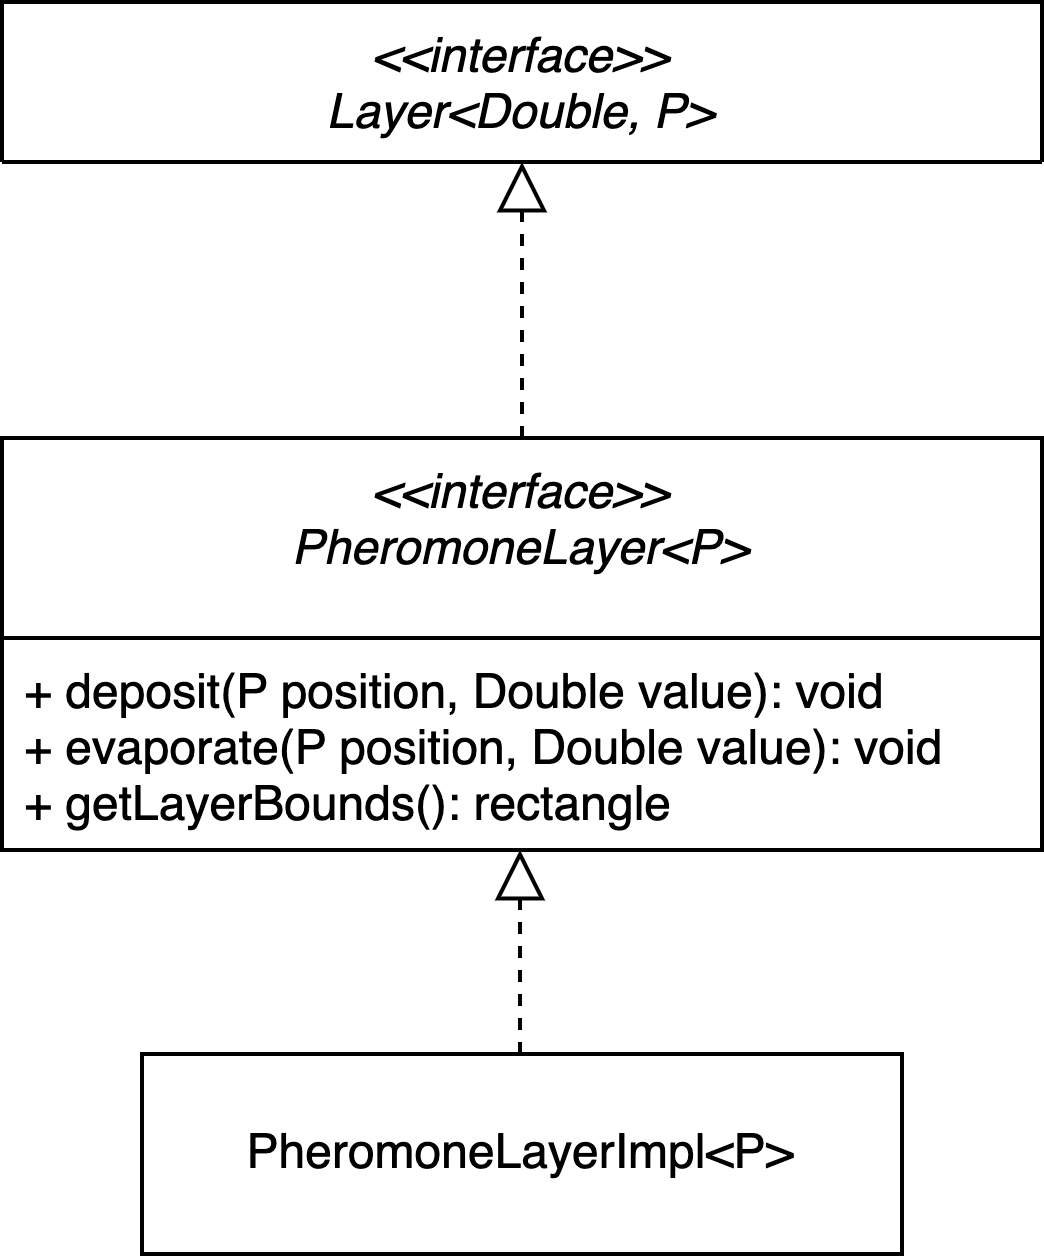
\includegraphics[width=.5\linewidth]{figures/pheromoneLayer.png}
    \caption{Struttura PheromoneLayer}\label{fig:phLayer}
\end{figure}
Il \texttt{PheromoneLayer<P extends Position2D<P>>}, layer personalizzato della simulazione, è stato implementato 
come un'interfaccia che estende \texttt{Layer<T, P>} - interfaccia propria di Alchemist -
dove \texttt{T} è il tipo di nodo e \texttt{P} è il tipo di posizione. 
L'utilizzo del parametro \texttt{P} implica che il \texttt{PheromoneLayer} può essere utilizzato con qualsiasi tipo di posizione, ma, nel contesto di questa tesi,
si è preferito sfruttare posizioni \texttt{Position2D<P>} bidimensionali.
Per la sua creazione è necessario definire 5 misure:
\begin{itemize}
    \item \texttt{startX}: la coordinata x di partenza.
    \item \texttt{startY}: la coordinata y di partenza.
    \item \texttt{width}: la larghezza del layer.
    \item \texttt{height}: l'altezza del layer.
    \item \texttt{step}: la dimensione del passo, ovvero la lunghezza del lato di ogni \textit{patch}.
\end{itemize}
Lo \texttt{step} è un parametro fondamentale per la corretta implementazione della simulazione
in quanto Alchemist non possiede il concetto di area, necessaria per individuare una \textit{patch}.
Queste vengono rappresentate come ``aree'' puntiformi, e la loro dimensione (ovvero la distanza di un punto dall'altro) è appunto definita da questo parametro.
Nella simulazione, il nodo deposita il feromone in una qualsiasi posizione, discreta e non obbligatoriamente intera, all'interno dei limiti dello spazio, e il \texttt{PheromoneLayer} 
si occupa di convertire questa posizione in una appartenente ad una \textit{patch}. 
Il \texttt{PheromoneLayer} esegue, quindi, un arrotondamento per eccesso o per difetto, in modo tale da ottenere la posizione della \textit{patch} più vicina.
\begin{figure}[ht]
    \centering
    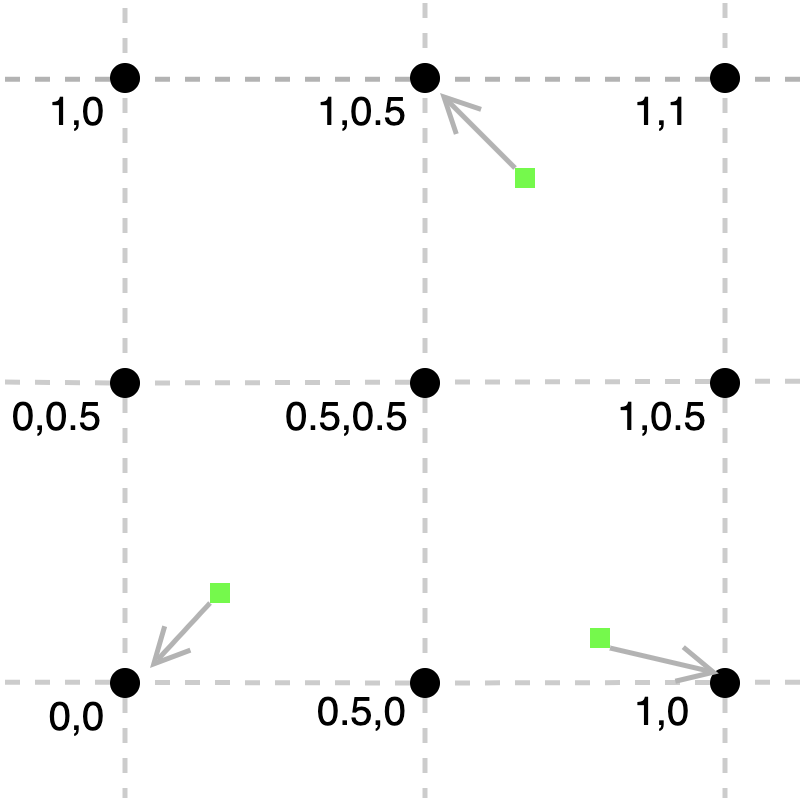
\includegraphics[width=.5\linewidth]{figures/patch-nodi.png}
    \caption{Rappresentazione grafica delle \textit{patches} puntiformi. Ogni punto rappresenta una patch,
    mentre i quadratini rappresentano i nodi e la freccia indica su che \textit{patch} il nodo depositerà il feromone. In questo esempio
    startX e startY hanno come valore 0, width e height 1 e step 0.5}\label{fig:patch-nodi}
\end{figure}
%devo parlare della Mappa e delle posizioni, di come vengono convertite magari aggiungendo delle foto.

\subsection{Struttura dati}
Un aspetto di fondamentale importanza riguarda la struttura dati utilizzata per la gestione del feromone.
Per ovviare alla mancanza del concetto di area, è stato utilizzato un \texttt{HashMap<P, Double>} che associa ad ogni posizione \texttt{P} un valore \texttt{Double} di feromone.
Questa mappa viene inizializzata nel costruttore della classe attraverso il metodo \texttt{setupEnviromnent()} che si occupa di popolare la mappa
con tutte le possibili posizioni delle \textit{patch} e di inizializzare il feromone a 0.\newline

\lstinputlisting[language=Java,label={lst:phlayer}]{listings/phlayersetup.java}

\subsection{Metodi}
I metodi definiti nell'interfaccia e implementati nella classe sono:
\begin{itemize}
    \item \texttt{void evaporate(P position, Double value)}: metodo che permette di far evaporare il feromone. 
    Richiede in input la posizione e il valore del feromone.
    \item \texttt{void deposit(P position, Double value)}: metodo che permette di depositare il feromone.
     Richiede in input la posizione e il valore del feromone.
    \item \texttt{Rectangle getLayerBounds()}: metodo che restituisce un oggetto di tipo \texttt{Rectangle}, contentente i parametri per delineare l'area del Layer.
\end{itemize}
Di grande importanza sono i primi due metodi: \texttt{evaporate} e \texttt{deposit}.
Entrambi sono nominati come le reazioni globali della simulazione e vengono utilizzati dalle stesse per accedere la mappa e modificare il feromone.\newline
\lstinputlisting[language=Java,label={lst:phlayer}]{listings/layer.java}

\section{Actions}
In questa sezione vengono descritte le azioni della simulazione. Possiamo trovare:
\begin{itemize}
    \item \texttt{MoveNode}: azione che permette ad ogni singolo nodo di muoversi.
    \item \texttt{NodeInfo}: azione che permette di controllare le informazioni di ogni singolo nodo.
\end{itemize}

\subsection{MoveNode}
La classe \texttt{MoveNode<P extends Position<P> \& Position2D<P>>} incorpora l'intera logica che permette il movimento di ogni singolo nodo. 
Per la sua creazione è necessario che l'utente definisca i seguenti parametri:
\begin{itemize}
    \item \texttt{sniffThreshold}: la soglia di feromone che il nodo deve percepire per potersi muovere.
    \item \texttt{sniffDistance}: la distanza del passo di movimento.
    \item \texttt{wiggleBias}: la tendenza a preferire un movimento casuale oscillatorio in una direzione specifica.
\end{itemize}
Il parametro \texttt{wiggleBias} può essere impostato in 3 modi:
\begin{itemize}
    \item \texttt{0}: il nodo ha il 50\% di muoversi in avanti e il 25\% di muoversi a destra o a sinistra.
    \item \texttt{0 > x <= 40}: il nodo tende a preferire la direzione di sinistra; il valore indica la probabilità di muoversi in quel verso.
    Il valore 40 indica il 100\% di probabilità di muoversi in quella direzione.
    \item \texttt{-40 => x < 0}: il nodo tende a preferire la direzione di destra; il valore indica la probabilità di muoversi in quel verso.
    Il valore -40 indica il 100\% di probabilità di muoversi in quella direzione.
\end{itemize}
La classe \texttt{MoveNode} estende la classe astratta \texttt{AbstractAction<T>}, facente parte del set base di Alchemist, implementandone i metodi astratti.
Tra questi, il metodo \texttt{execute} è il più importante, in quanto si occupa di eseguire l'azione di movimento vera e propria.
La logica di movimento segue questi passi:
\begin{enumerate}
    \item Viene individuata la posizione attuale del nodo.
    \item Questa posizione viene adattata alla \textit{patch} più vicina.
    \item Vengono calcolate le direzioni possibili in base alle patch adiacenti alla posizione calcolata precedentemente che hanno una 
    concentrazione di feromone superiore ad una soglia definita dall'utente (il parametro si chiama \texttt{sniffThreshold}).
    \item Viene identificata la \textit{patch} con la maggiore concentrazione di feromone. Tuttavia, questa, non è sempre individuabile. Vi sono due casi possibili: nel primo, 
        nella \textit{patch} è presente un valore di feromone, ma esso è sotto la soglia minima \texttt{sniffThreshold} e dunque la \textit{patch} viene scartata;
         nel secondo caso, invece, nella \textit{patch} non è presente alcuna traccia di feromone, e dunque questa non viene proprio rilevata.
    \item Se la \textit{patch} è presente:
    \begin{enumerate}
        \item La direzione del nodo viene aggiornata in base alla direzione della \textit{patch} con la maggiore concentrazione di feromone.
        \item Il nodo si muove verso quella \textit{patch} e si aggiorna la direzione del nodo.
    \end{enumerate}
    \item Se la \textit{patch} non è presente:
    \begin{enumerate}
        \item Viene calcolata una direzione casuale tra quelle possibili (dritto, verso destra o verso sinistra a seconda del valore del parametro \texttt{wiggleBias}),
        tenendo in considerazione la direzione attuale del nodo.
        \item Il nodo si muove nella direzione scelta e l'orientamento del nodo viene aggiornato.
    \end{enumerate}
\end{enumerate}

\subsection{NodeInfo}
La classe \texttt{NodeInfo<T, P extends Position<P> \& Position2D<P>>} permette di tracciare le informazioni di ogni singolo nodo. Anche questa
classe estende la classe astratta \texttt{AbstractAction<T>}, implementandone i metodi. Le informazioni osservabili sono le seguenti:
\begin{itemize}
    \item \texttt{PheromoneValue}: la concentrazione di feromone nella \textit{patch} in cui si trova il nodo.
    \item \texttt{direction}: la direzione attuale del nodo.
    \item \texttt{pheromone}: la quantità di feromone che il nodo rilascia.
\end{itemize}

\begin{figure}[ht]
    \centering
    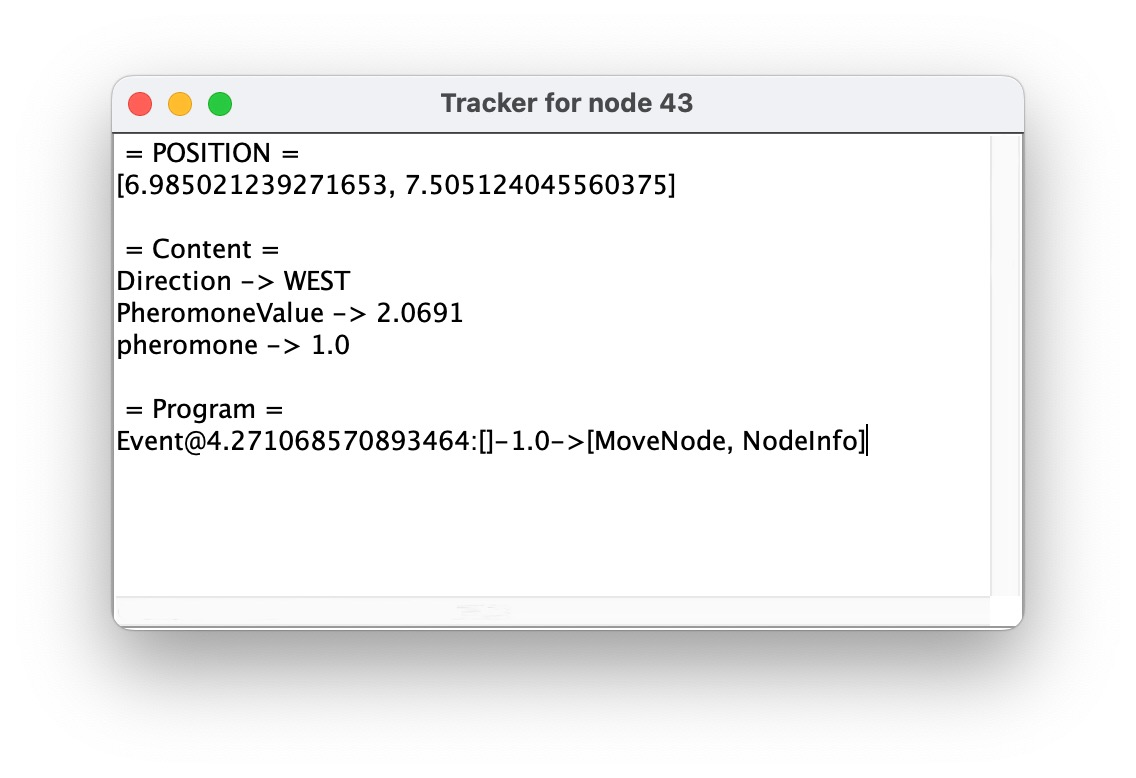
\includegraphics[width=.7\linewidth]{figures/nodeinfo.jpg}
    \caption{Le informazioni del nodo. Si possono osservare nella sezione ``Content''}\label{fig:nodeinfo}
\end{figure}

\section{GlobalReactions}
\begin{figure}[ht]
    \centering
    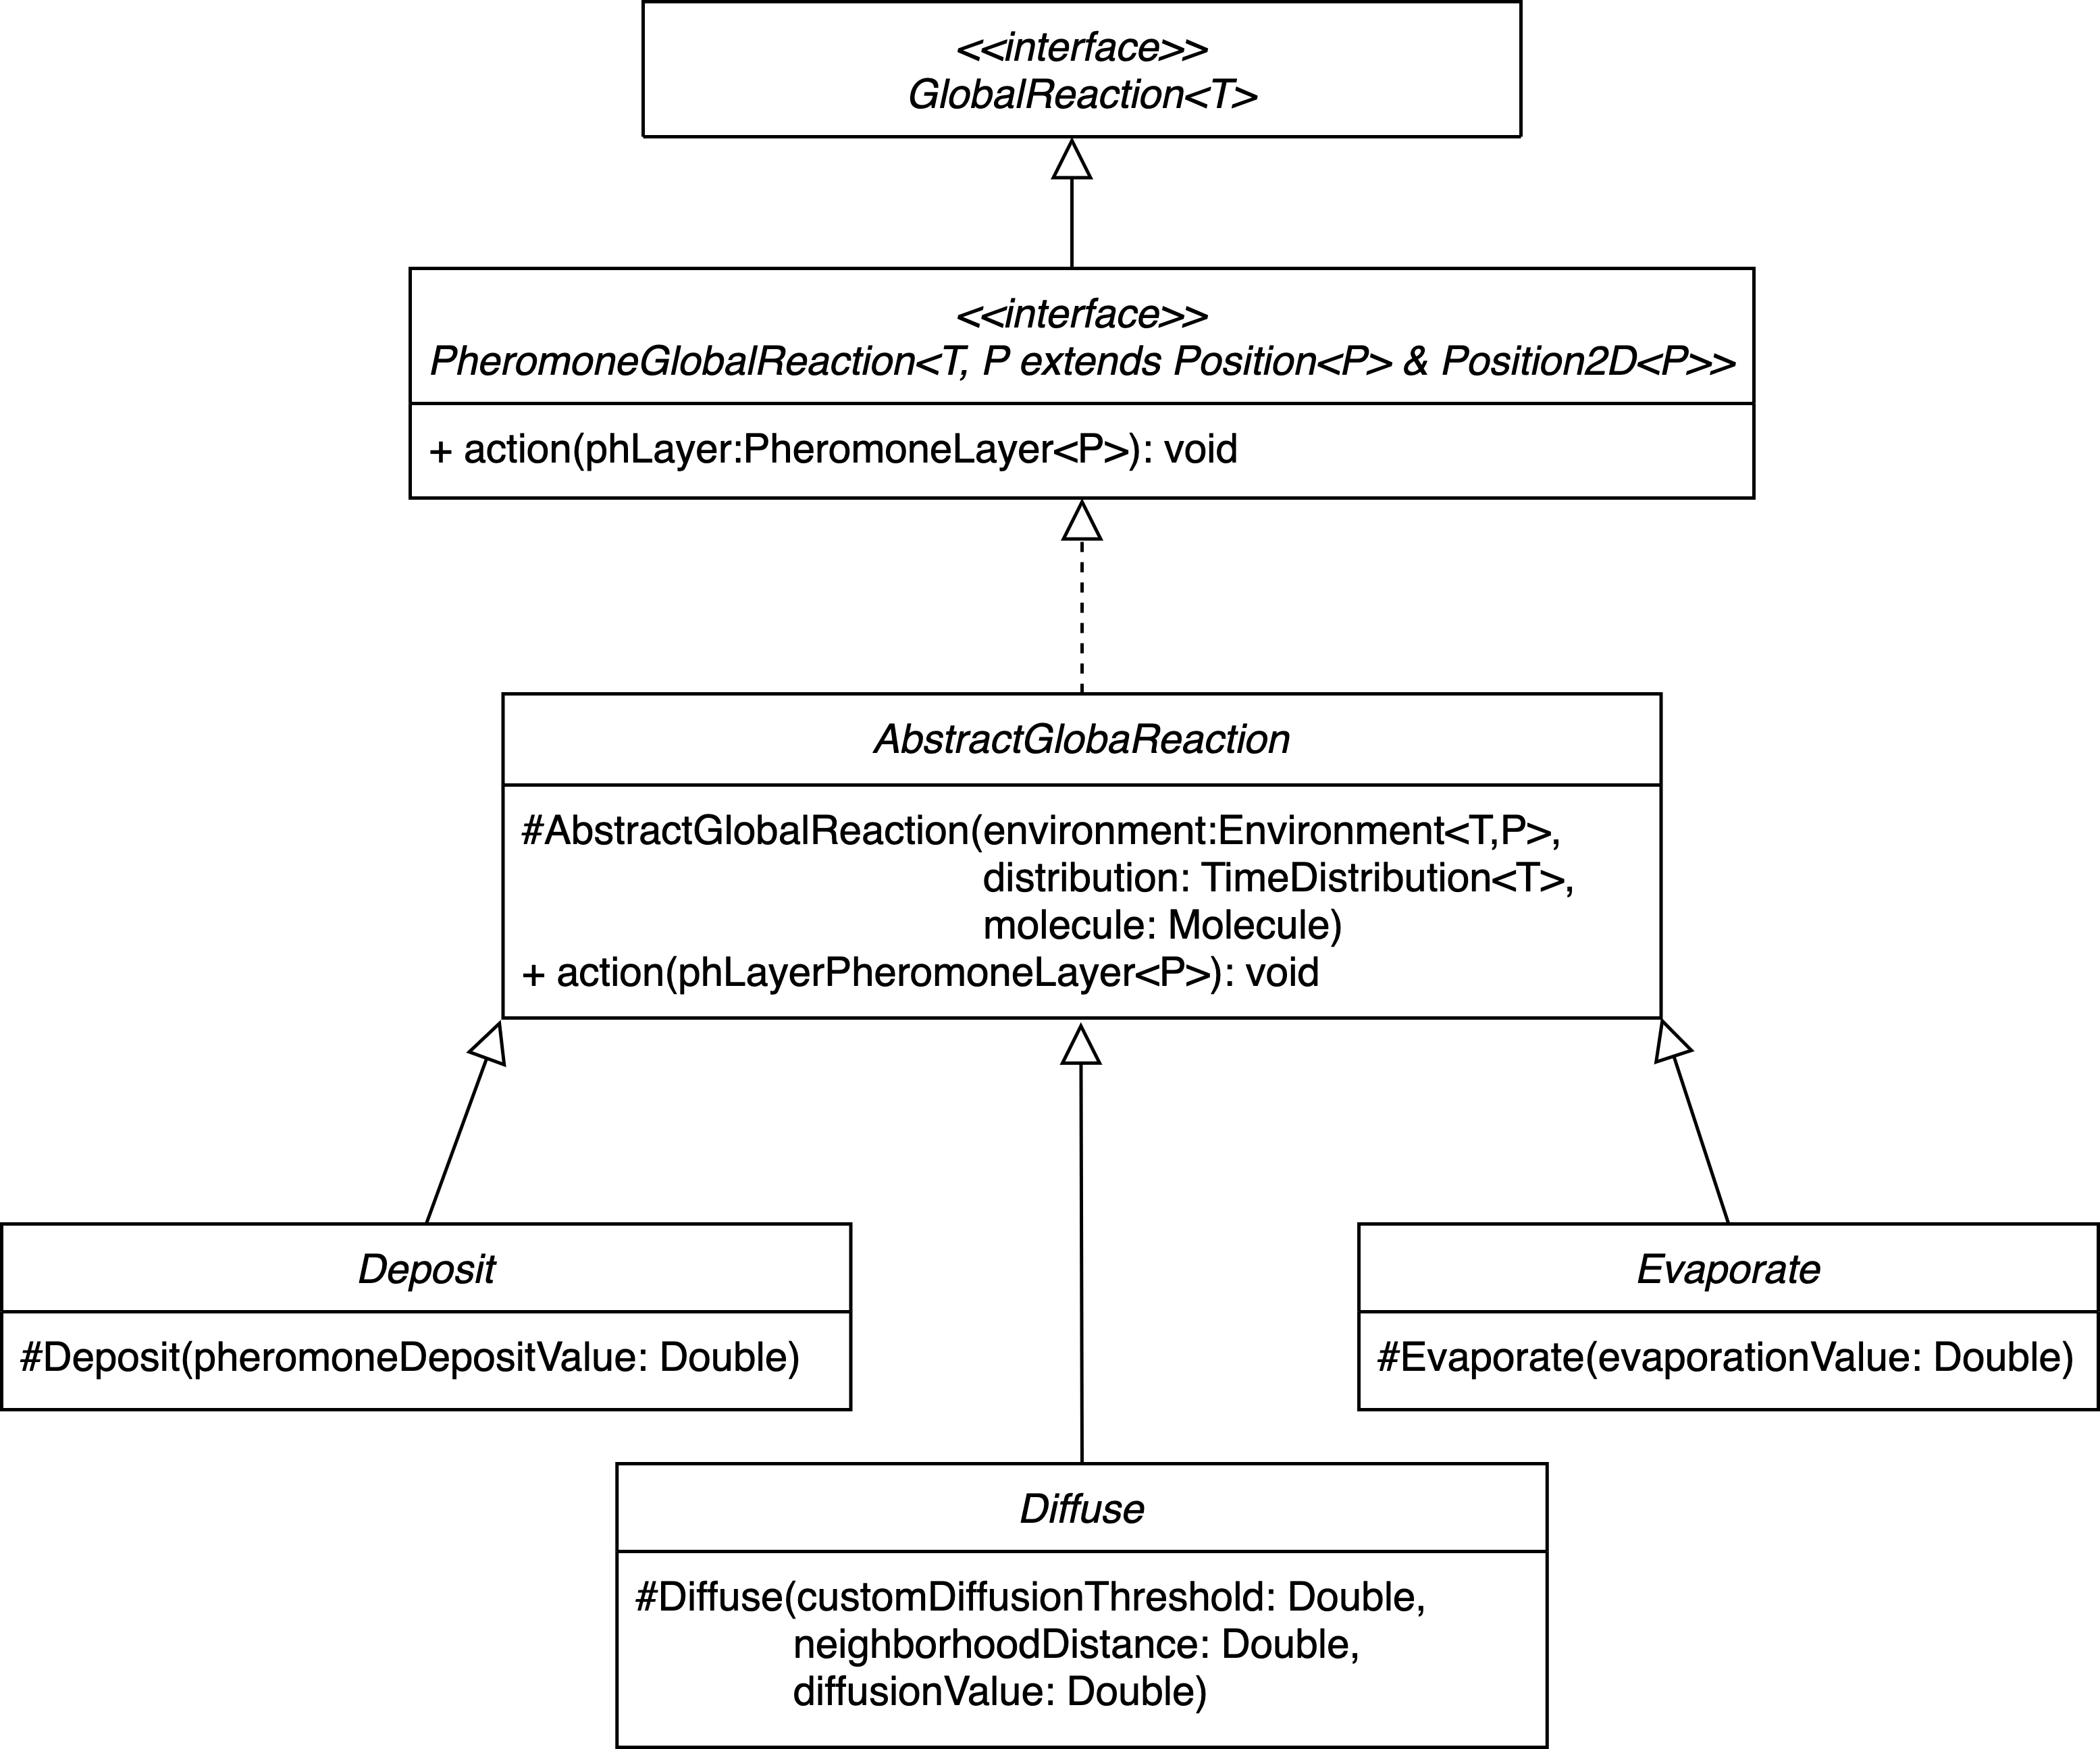
\includegraphics[width=.7\linewidth]{figures/global.png}
    \caption{Schema delle Global Reaction }\label{fig:global}
\end{figure}
In questa sezione del progetto sono state implementate le azioni globali della simulazione. Possiamo trovare:
\begin{itemize}
    \item \texttt{Evaporate}: azione che permette di far evaporare il feromone.
    \item \texttt{Deposit}: azione che permette di far diffondere il feromone.
    \item \texttt{Diffuse}: azione che diffonde il feromone nelle patch adiacenti.
\end{itemize}
